% This file is generated by the MATLAB m-file laprint.m. It can be included
% into LaTeX documents using the packages graphicx, color and psfrag.
% It is accompanied by a postscript file. A sample LaTeX file is:
%    \documentclass{article}\usepackage{graphicx,color,psfrag}
%    \begin{document}% This file is generated by the MATLAB m-file laprint.m. It can be included
% into LaTeX documents using the packages graphicx, color and psfrag.
% It is accompanied by a postscript file. A sample LaTeX file is:
%    \documentclass{article}\usepackage{graphicx,color,psfrag}
%    \begin{document}% This file is generated by the MATLAB m-file laprint.m. It can be included
% into LaTeX documents using the packages graphicx, color and psfrag.
% It is accompanied by a postscript file. A sample LaTeX file is:
%    \documentclass{article}\usepackage{graphicx,color,psfrag}
%    \begin{document}% This file is generated by the MATLAB m-file laprint.m. It can be included
% into LaTeX documents using the packages graphicx, color and psfrag.
% It is accompanied by a postscript file. A sample LaTeX file is:
%    \documentclass{article}\usepackage{graphicx,color,psfrag}
%    \begin{document}\input{compL2}\end{document}
% See http://www.mathworks.de/matlabcentral/fileexchange/loadFile.do?objectId=4638
% for recent versions of laprint.m.
%
% created by:           LaPrint version 3.16 (13.9.2004)
% created on:           29-May-2012 16:31:49
% eps bounding box:     15 cm x 11.1094 cm
% comment:              
%
\begin{psfrags}%
\psfragscanon%
%
% text strings:
\psfrag{s05}[t][t]{\color[rgb]{0,0,0}\setlength{\tabcolsep}{0pt}\begin{tabular}{c}$M$\end{tabular}}%
\psfrag{s06}[b][b][1][180]{\color[rgb]{0,0,0}\setlength{\tabcolsep}{0pt}\begin{tabular}{c}$\epsilon_{2}$
error\end{tabular}}%
\psfrag{s12}[l][l]{\color[rgb]{0,0,0}quasi-bicubic}%
\psfrag{s17}[l][l]{\color[rgb]{0,0,0}$\tpbs^0_p$}%
\psfrag{s18}[l][l]{\color[rgb]{0,0,0}$\tpbs^1_p$ interp.}%
\psfrag{s19}[l][l]{\color[rgb]{0,0,0}Collatz - Keys bicubic}%
\psfrag{s20}[l][l]{\color[rgb]{0,0,0}$\tpbs^3$ interp.}%
\psfrag{s21}[l][l]{\color[rgb]{0,0,0}$\tpbs^3$ quasi.}%
%
% slopes
\psfrag{u1}[r][r]{\color[rgb]{0,0,0}$1.0007$}%
\psfrag{u2}[r][r]{\color[rgb]{0,0,0}$1.9996$}%
\psfrag{u3}[r][r]{\color[rgb]{0,0,0}$3.0165$}%
\psfrag{u4}[r][r]{\color[rgb]{0,0,0}$3.9823$}%
\psfrag{u5}[r][r]{\color[rgb]{0,0,0}$4.0169$}%

%
% xticklabels:
\psfrag{x01}[t][t]{0}%
\psfrag{x02}[t][t]{0.1}%
\psfrag{x03}[t][t]{0.2}%
\psfrag{x04}[t][t]{0.3}%
\psfrag{x05}[t][t]{0.4}%
\psfrag{x06}[t][t]{0.5}%
\psfrag{x07}[t][t]{0.6}%
\psfrag{x08}[t][t]{0.7}%
\psfrag{x09}[t][t]{0.8}%
\psfrag{x10}[t][t]{0.9}%
\psfrag{x11}[t][t]{1}%
\psfrag{x12}[t][t]{${32}$}%
\psfrag{x13}[t][t]{${64}$}%
\psfrag{x14}[t][t]{${128}$}%
\psfrag{x15}[t][t]{${256}$}%
\psfrag{x16}[t][t]{${512}$}%
\psfrag{x17}[t][t]{${1024}$}%
%
% yticklabels:
\psfrag{v01}[r][r]{0}%
\psfrag{v02}[r][r]{0.1}%
\psfrag{v03}[r][r]{0.2}%
\psfrag{v04}[r][r]{0.3}%
\psfrag{v05}[r][r]{0.4}%
\psfrag{v06}[r][r]{0.5}%
\psfrag{v07}[r][r]{0.6}%
\psfrag{v08}[r][r]{0.7}%
\psfrag{v09}[r][r]{0.8}%
\psfrag{v10}[r][r]{0.9}%
\psfrag{v11}[r][r]{1}%
\psfrag{v12}[r][r]{$10^{-8}$}%
\psfrag{v13}[r][r]{$10^{-7}$}%
\psfrag{v14}[r][r]{$10^{-6}$}%
\psfrag{v15}[r][r]{$10^{-5}$}%
\psfrag{v16}[r][r]{$10^{-4}$}%
\psfrag{v17}[r][r]{$10^{-3}$}%
\psfrag{v18}[r][r]{$10^{-2}$}%
\psfrag{v19}[r][r]{$10^{-1}$}%
\psfrag{v20}[r][r]{$10^{0}$}%
\psfrag{v21}[r][r]{$10^{1}$}%
%
% Figure:
\resizebox{6cm}{!}{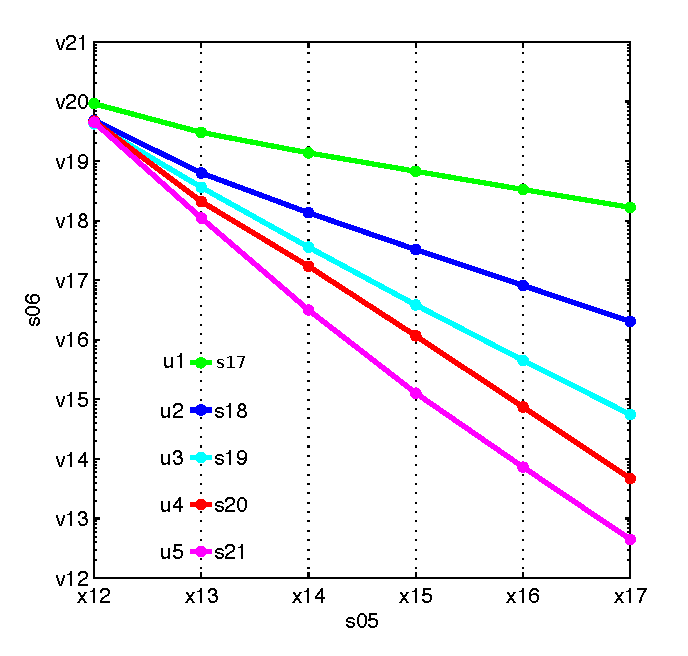
\includegraphics{compL2.eps}}%
\end{psfrags}%
%
% End compL2.tex
\end{document}
% See http://www.mathworks.de/matlabcentral/fileexchange/loadFile.do?objectId=4638
% for recent versions of laprint.m.
%
% created by:           LaPrint version 3.16 (13.9.2004)
% created on:           29-May-2012 16:31:49
% eps bounding box:     15 cm x 11.1094 cm
% comment:              
%
\begin{psfrags}%
\psfragscanon%
%
% text strings:
\psfrag{s05}[t][t]{\color[rgb]{0,0,0}\setlength{\tabcolsep}{0pt}\begin{tabular}{c}$M$\end{tabular}}%
\psfrag{s06}[b][b][1][180]{\color[rgb]{0,0,0}\setlength{\tabcolsep}{0pt}\begin{tabular}{c}$\epsilon_{2}$
error\end{tabular}}%
\psfrag{s12}[l][l]{\color[rgb]{0,0,0}quasi-bicubic}%
\psfrag{s17}[l][l]{\color[rgb]{0,0,0}$\tpbs^0_p$}%
\psfrag{s18}[l][l]{\color[rgb]{0,0,0}$\tpbs^1_p$ interp.}%
\psfrag{s19}[l][l]{\color[rgb]{0,0,0}Collatz - Keys bicubic}%
\psfrag{s20}[l][l]{\color[rgb]{0,0,0}$\tpbs^3$ interp.}%
\psfrag{s21}[l][l]{\color[rgb]{0,0,0}$\tpbs^3$ quasi.}%
%
% slopes
\psfrag{u1}[r][r]{\color[rgb]{0,0,0}$1.0007$}%
\psfrag{u2}[r][r]{\color[rgb]{0,0,0}$1.9996$}%
\psfrag{u3}[r][r]{\color[rgb]{0,0,0}$3.0165$}%
\psfrag{u4}[r][r]{\color[rgb]{0,0,0}$3.9823$}%
\psfrag{u5}[r][r]{\color[rgb]{0,0,0}$4.0169$}%

%
% xticklabels:
\psfrag{x01}[t][t]{0}%
\psfrag{x02}[t][t]{0.1}%
\psfrag{x03}[t][t]{0.2}%
\psfrag{x04}[t][t]{0.3}%
\psfrag{x05}[t][t]{0.4}%
\psfrag{x06}[t][t]{0.5}%
\psfrag{x07}[t][t]{0.6}%
\psfrag{x08}[t][t]{0.7}%
\psfrag{x09}[t][t]{0.8}%
\psfrag{x10}[t][t]{0.9}%
\psfrag{x11}[t][t]{1}%
\psfrag{x12}[t][t]{${32}$}%
\psfrag{x13}[t][t]{${64}$}%
\psfrag{x14}[t][t]{${128}$}%
\psfrag{x15}[t][t]{${256}$}%
\psfrag{x16}[t][t]{${512}$}%
\psfrag{x17}[t][t]{${1024}$}%
%
% yticklabels:
\psfrag{v01}[r][r]{0}%
\psfrag{v02}[r][r]{0.1}%
\psfrag{v03}[r][r]{0.2}%
\psfrag{v04}[r][r]{0.3}%
\psfrag{v05}[r][r]{0.4}%
\psfrag{v06}[r][r]{0.5}%
\psfrag{v07}[r][r]{0.6}%
\psfrag{v08}[r][r]{0.7}%
\psfrag{v09}[r][r]{0.8}%
\psfrag{v10}[r][r]{0.9}%
\psfrag{v11}[r][r]{1}%
\psfrag{v12}[r][r]{$10^{-8}$}%
\psfrag{v13}[r][r]{$10^{-7}$}%
\psfrag{v14}[r][r]{$10^{-6}$}%
\psfrag{v15}[r][r]{$10^{-5}$}%
\psfrag{v16}[r][r]{$10^{-4}$}%
\psfrag{v17}[r][r]{$10^{-3}$}%
\psfrag{v18}[r][r]{$10^{-2}$}%
\psfrag{v19}[r][r]{$10^{-1}$}%
\psfrag{v20}[r][r]{$10^{0}$}%
\psfrag{v21}[r][r]{$10^{1}$}%
%
% Figure:
\resizebox{6cm}{!}{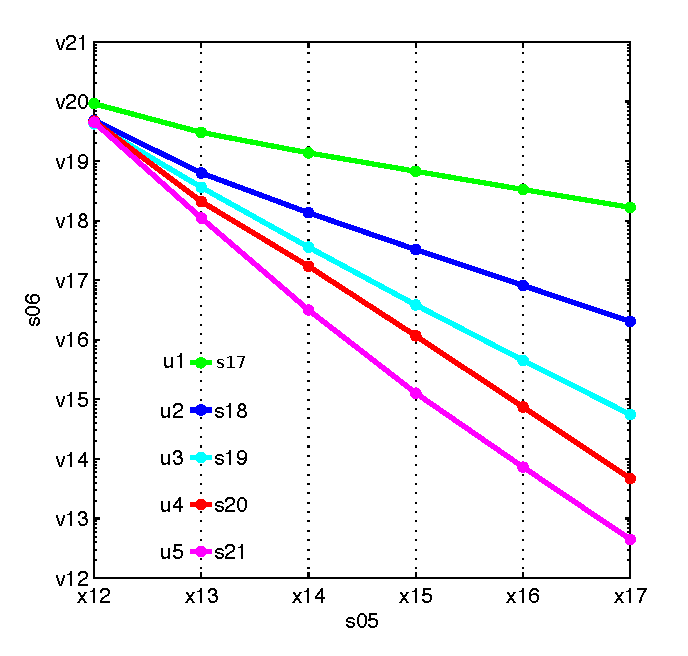
\includegraphics{compL2.eps}}%
\end{psfrags}%
%
% End compL2.tex
\end{document}
% See http://www.mathworks.de/matlabcentral/fileexchange/loadFile.do?objectId=4638
% for recent versions of laprint.m.
%
% created by:           LaPrint version 3.16 (13.9.2004)
% created on:           29-May-2012 16:31:49
% eps bounding box:     15 cm x 11.1094 cm
% comment:              
%
\begin{psfrags}%
\psfragscanon%
%
% text strings:
\psfrag{s05}[t][t]{\color[rgb]{0,0,0}\setlength{\tabcolsep}{0pt}\begin{tabular}{c}$M$\end{tabular}}%
\psfrag{s06}[b][b][1][180]{\color[rgb]{0,0,0}\setlength{\tabcolsep}{0pt}\begin{tabular}{c}$\epsilon_{2}$
error\end{tabular}}%
\psfrag{s12}[l][l]{\color[rgb]{0,0,0}quasi-bicubic}%
\psfrag{s17}[l][l]{\color[rgb]{0,0,0}$\tpbs^0_p$}%
\psfrag{s18}[l][l]{\color[rgb]{0,0,0}$\tpbs^1_p$ interp.}%
\psfrag{s19}[l][l]{\color[rgb]{0,0,0}Collatz - Keys bicubic}%
\psfrag{s20}[l][l]{\color[rgb]{0,0,0}$\tpbs^3$ interp.}%
\psfrag{s21}[l][l]{\color[rgb]{0,0,0}$\tpbs^3$ quasi.}%
%
% slopes
\psfrag{u1}[r][r]{\color[rgb]{0,0,0}$1.0007$}%
\psfrag{u2}[r][r]{\color[rgb]{0,0,0}$1.9996$}%
\psfrag{u3}[r][r]{\color[rgb]{0,0,0}$3.0165$}%
\psfrag{u4}[r][r]{\color[rgb]{0,0,0}$3.9823$}%
\psfrag{u5}[r][r]{\color[rgb]{0,0,0}$4.0169$}%

%
% xticklabels:
\psfrag{x01}[t][t]{0}%
\psfrag{x02}[t][t]{0.1}%
\psfrag{x03}[t][t]{0.2}%
\psfrag{x04}[t][t]{0.3}%
\psfrag{x05}[t][t]{0.4}%
\psfrag{x06}[t][t]{0.5}%
\psfrag{x07}[t][t]{0.6}%
\psfrag{x08}[t][t]{0.7}%
\psfrag{x09}[t][t]{0.8}%
\psfrag{x10}[t][t]{0.9}%
\psfrag{x11}[t][t]{1}%
\psfrag{x12}[t][t]{${32}$}%
\psfrag{x13}[t][t]{${64}$}%
\psfrag{x14}[t][t]{${128}$}%
\psfrag{x15}[t][t]{${256}$}%
\psfrag{x16}[t][t]{${512}$}%
\psfrag{x17}[t][t]{${1024}$}%
%
% yticklabels:
\psfrag{v01}[r][r]{0}%
\psfrag{v02}[r][r]{0.1}%
\psfrag{v03}[r][r]{0.2}%
\psfrag{v04}[r][r]{0.3}%
\psfrag{v05}[r][r]{0.4}%
\psfrag{v06}[r][r]{0.5}%
\psfrag{v07}[r][r]{0.6}%
\psfrag{v08}[r][r]{0.7}%
\psfrag{v09}[r][r]{0.8}%
\psfrag{v10}[r][r]{0.9}%
\psfrag{v11}[r][r]{1}%
\psfrag{v12}[r][r]{$10^{-8}$}%
\psfrag{v13}[r][r]{$10^{-7}$}%
\psfrag{v14}[r][r]{$10^{-6}$}%
\psfrag{v15}[r][r]{$10^{-5}$}%
\psfrag{v16}[r][r]{$10^{-4}$}%
\psfrag{v17}[r][r]{$10^{-3}$}%
\psfrag{v18}[r][r]{$10^{-2}$}%
\psfrag{v19}[r][r]{$10^{-1}$}%
\psfrag{v20}[r][r]{$10^{0}$}%
\psfrag{v21}[r][r]{$10^{1}$}%
%
% Figure:
\resizebox{6cm}{!}{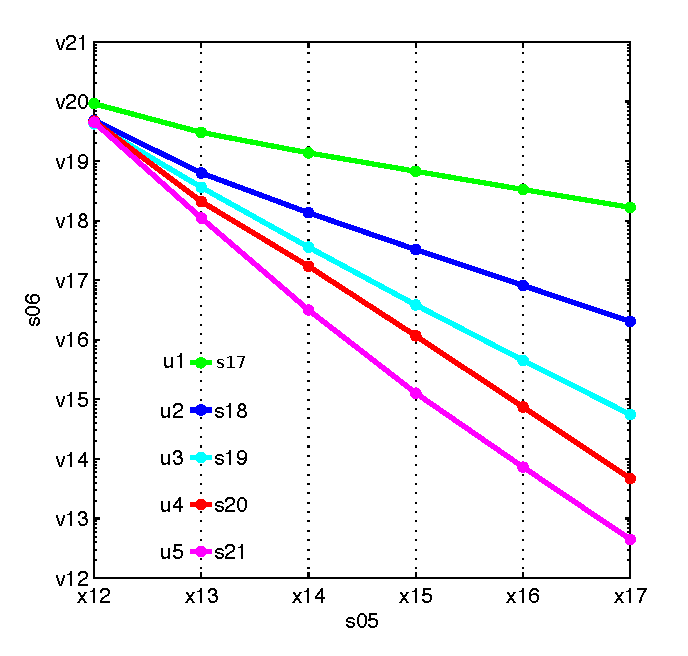
\includegraphics{compL2.eps}}%
\end{psfrags}%
%
% End compL2.tex
\end{document}
% See http://www.mathworks.de/matlabcentral/fileexchange/loadFile.do?objectId=4638
% for recent versions of laprint.m.
%
% created by:           LaPrint version 3.16 (13.9.2004)
% created on:           29-May-2012 16:31:49
% eps bounding box:     15 cm x 11.1094 cm
% comment:              
%
\begin{psfrags}%
\psfragscanon%
%
% text strings:
\psfrag{s05}[t][t]{\color[rgb]{0,0,0}\setlength{\tabcolsep}{0pt}\begin{tabular}{c}$M$\end{tabular}}%
\psfrag{s06}[b][b][1][180]{\color[rgb]{0,0,0}\setlength{\tabcolsep}{0pt}\begin{tabular}{c}$\epsilon_{2}$
error\end{tabular}}%
\psfrag{s12}[l][l]{\color[rgb]{0,0,0}quasi-bicubic}%
\psfrag{s17}[l][l]{\color[rgb]{0,0,0}$\tpbs^0_p$}%
\psfrag{s18}[l][l]{\color[rgb]{0,0,0}$\tpbs^1_p$ interp.}%
\psfrag{s19}[l][l]{\color[rgb]{0,0,0}Collatz - Keys bicubic}%
\psfrag{s20}[l][l]{\color[rgb]{0,0,0}$\tpbs^3$ interp.}%
\psfrag{s21}[l][l]{\color[rgb]{0,0,0}$\tpbs^3$ quasi.}%
%
% slopes
\psfrag{u1}[r][r]{\color[rgb]{0,0,0}$1.0007$}%
\psfrag{u2}[r][r]{\color[rgb]{0,0,0}$1.9996$}%
\psfrag{u3}[r][r]{\color[rgb]{0,0,0}$3.0165$}%
\psfrag{u4}[r][r]{\color[rgb]{0,0,0}$3.9823$}%
\psfrag{u5}[r][r]{\color[rgb]{0,0,0}$4.0169$}%

%
% xticklabels:
\psfrag{x01}[t][t]{0}%
\psfrag{x02}[t][t]{0.1}%
\psfrag{x03}[t][t]{0.2}%
\psfrag{x04}[t][t]{0.3}%
\psfrag{x05}[t][t]{0.4}%
\psfrag{x06}[t][t]{0.5}%
\psfrag{x07}[t][t]{0.6}%
\psfrag{x08}[t][t]{0.7}%
\psfrag{x09}[t][t]{0.8}%
\psfrag{x10}[t][t]{0.9}%
\psfrag{x11}[t][t]{1}%
\psfrag{x12}[t][t]{${32}$}%
\psfrag{x13}[t][t]{${64}$}%
\psfrag{x14}[t][t]{${128}$}%
\psfrag{x15}[t][t]{${256}$}%
\psfrag{x16}[t][t]{${512}$}%
\psfrag{x17}[t][t]{${1024}$}%
%
% yticklabels:
\psfrag{v01}[r][r]{0}%
\psfrag{v02}[r][r]{0.1}%
\psfrag{v03}[r][r]{0.2}%
\psfrag{v04}[r][r]{0.3}%
\psfrag{v05}[r][r]{0.4}%
\psfrag{v06}[r][r]{0.5}%
\psfrag{v07}[r][r]{0.6}%
\psfrag{v08}[r][r]{0.7}%
\psfrag{v09}[r][r]{0.8}%
\psfrag{v10}[r][r]{0.9}%
\psfrag{v11}[r][r]{1}%
\psfrag{v12}[r][r]{$10^{-8}$}%
\psfrag{v13}[r][r]{$10^{-7}$}%
\psfrag{v14}[r][r]{$10^{-6}$}%
\psfrag{v15}[r][r]{$10^{-5}$}%
\psfrag{v16}[r][r]{$10^{-4}$}%
\psfrag{v17}[r][r]{$10^{-3}$}%
\psfrag{v18}[r][r]{$10^{-2}$}%
\psfrag{v19}[r][r]{$10^{-1}$}%
\psfrag{v20}[r][r]{$10^{0}$}%
\psfrag{v21}[r][r]{$10^{1}$}%
%
% Figure:
\resizebox{6cm}{!}{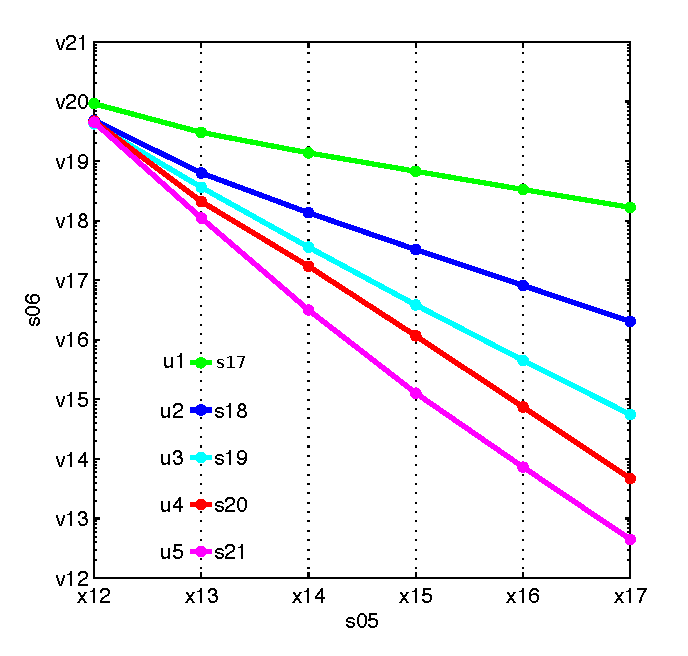
\includegraphics{compL2.eps}}%
\end{psfrags}%
%
% End compL2.tex
